\chapter{Analisi delle centralità}

\section{Obiettivi dell’analisi}

Dopo aver descritto la struttura generale della rete tramite l’analisi esplorativa, il passo successivo consiste nello studio delle misure di centralità. Queste misure permettono di valutare l’importanza dei nodi non soltanto in base al numero di connessioni, ma anche in funzione del loro ruolo strutturale all’interno della rete.

Nel caso della rete delle rotte aeree, l’analisi delle centralità consente di individuare aeroporti con caratteristiche differenti: nodi in grado di collegare porzioni diverse della rete, aeroporti particolarmente vicini al resto del sistema e scali che risultano strutturalmente rilevanti in virtù della qualità delle connessioni ricevute. In questo progetto sono state considerate quattro misure principali:
\begin{itemize}
    \item \textbf{betweenness centrality}, per individuare i nodi con maggiore capacità di intermediazione;
    \item \textbf{closeness centrality}, per evidenziare gli aeroporti mediamente più vicini al resto della rete;
    \item \textbf{PageRank}, per misurare l’importanza di un nodo tenendo conto anche della rilevanza dei collegamenti ricevuti;
    \item \textbf{eigenvector centrality}, per individuare i nodi connessi ad altri nodi a loro volta molto centrali.
\end{itemize}

Poiché il grafo presenta dimensioni elevate, la betweenness centrality è stata calcolata tramite una procedura approssimata basata su campionamento, con parametro \(k=200\), mentre la closeness e il PageRank sono stati calcolati sulla largest weakly connected component del grafo diretto. Per il PageRank è stato inoltre mantenuto il peso degli archi, definito come numero di compagnie aeree distinte che operano una determinata rotta. L’eigenvector centrality è stata invece calcolata sulla versione non diretta della largest weakly connected component, così da ottenere una misura più stabile e interpretabile del prestigio strutturale dei nodi.

\section{Betweenness centrality}

La betweenness centrality misura quante volte un nodo si colloca sui cammini minimi che collegano coppie di nodi della rete. In termini applicativi, essa consente di individuare aeroporti che svolgono un ruolo di \textit{ponte} tra aree differenti del sistema di trasporto aereo.

\begin{figure}[H]
\centering
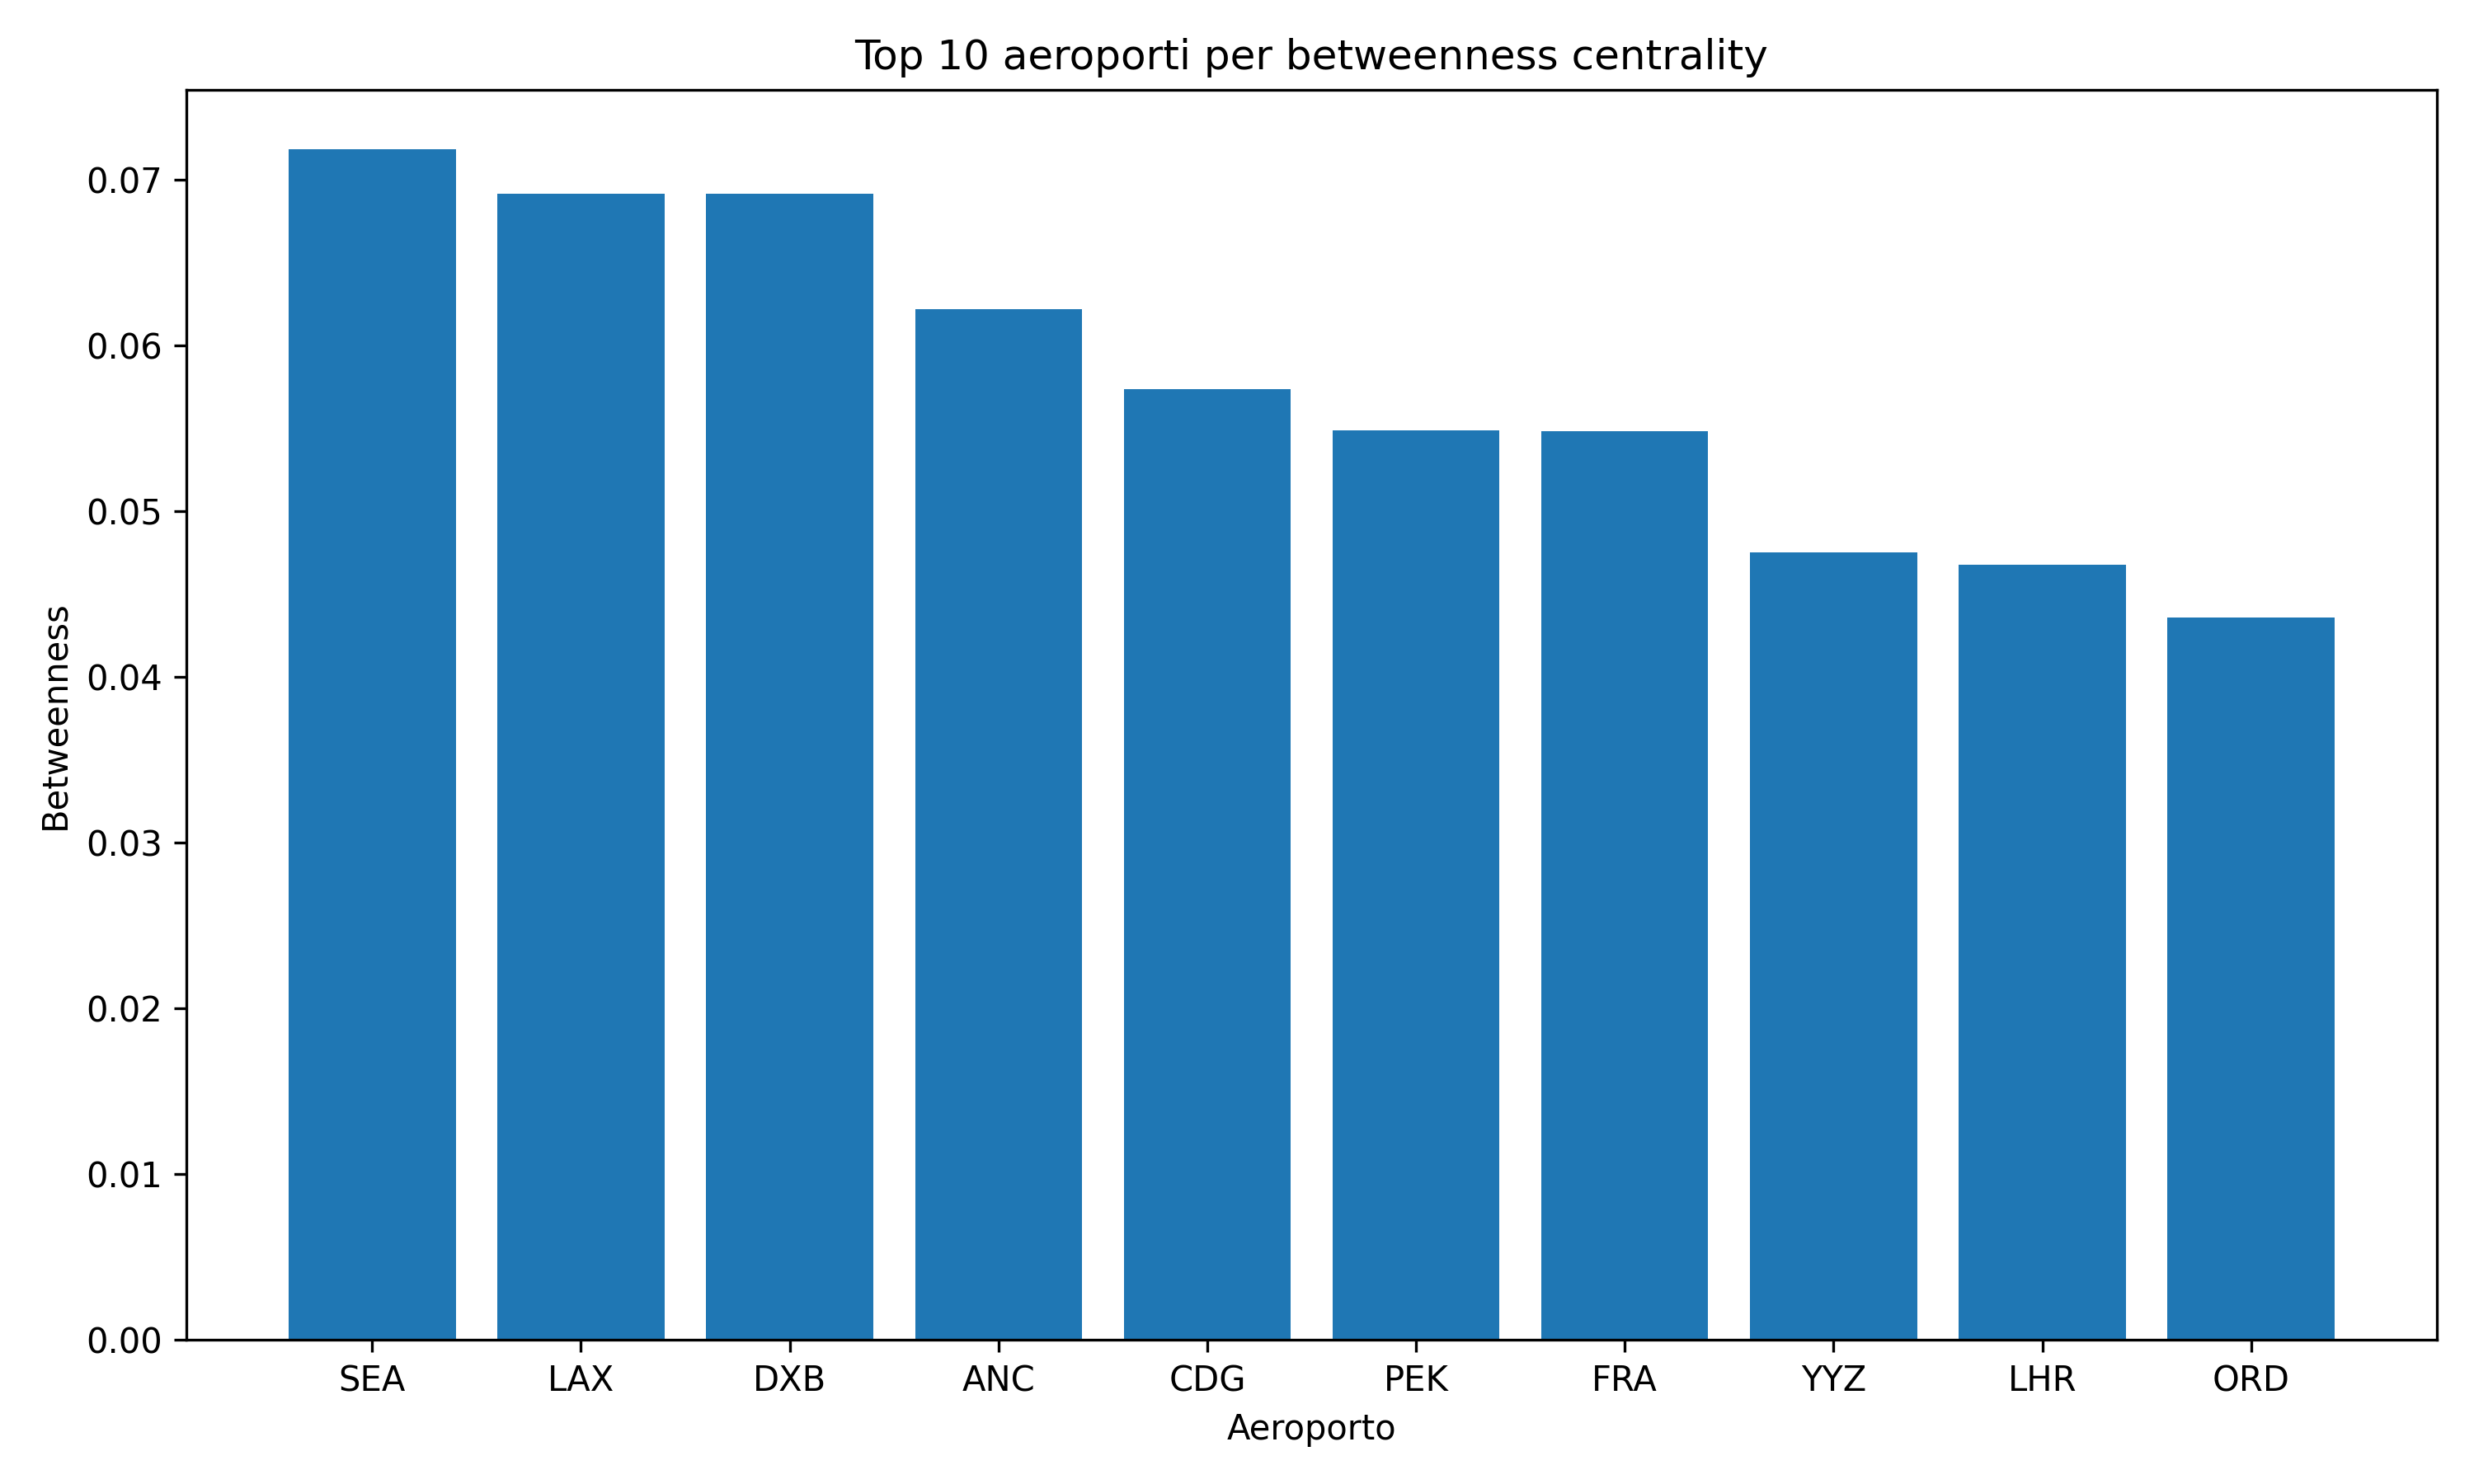
\includegraphics[width=0.9\textwidth]{chapter5/immagini/top10_betweenness.png}
\caption{Top 10 aeroporti per betweenness centrality.}
\label{fig:top_betweenness}
\end{figure}

Come mostrato nella Figura~\ref{fig:top_betweenness}, gli aeroporti con i valori più elevati di betweenness sono SEA, LAX, DXB, ANC, CDG, PEK, FRA, YYZ, LHR e ORD. Il risultato è particolarmente interessante perché non coincide perfettamente con il ranking dei nodi a maggior grado osservato nel capitolo precedente.

Questo aspetto suggerisce che la centralità di intermediazione non dipende soltanto dal numero di collegamenti diretti, ma soprattutto dalla posizione strategica del nodo nei percorsi della rete. Aeroporti come SEA, LAX e DXB emergono infatti come punti di passaggio rilevanti tra differenti porzioni del sistema, svolgendo un ruolo di connessione tra aree che altrimenti risulterebbero meno direttamente collegate.

Per osservare in modo più immediato le relazioni tra i nodi più rilevanti secondo questa misura, è stato costruito anche il sottografo dei primi 20 aeroporti per betweenness centrality.

\begin{figure}[H]
\centering
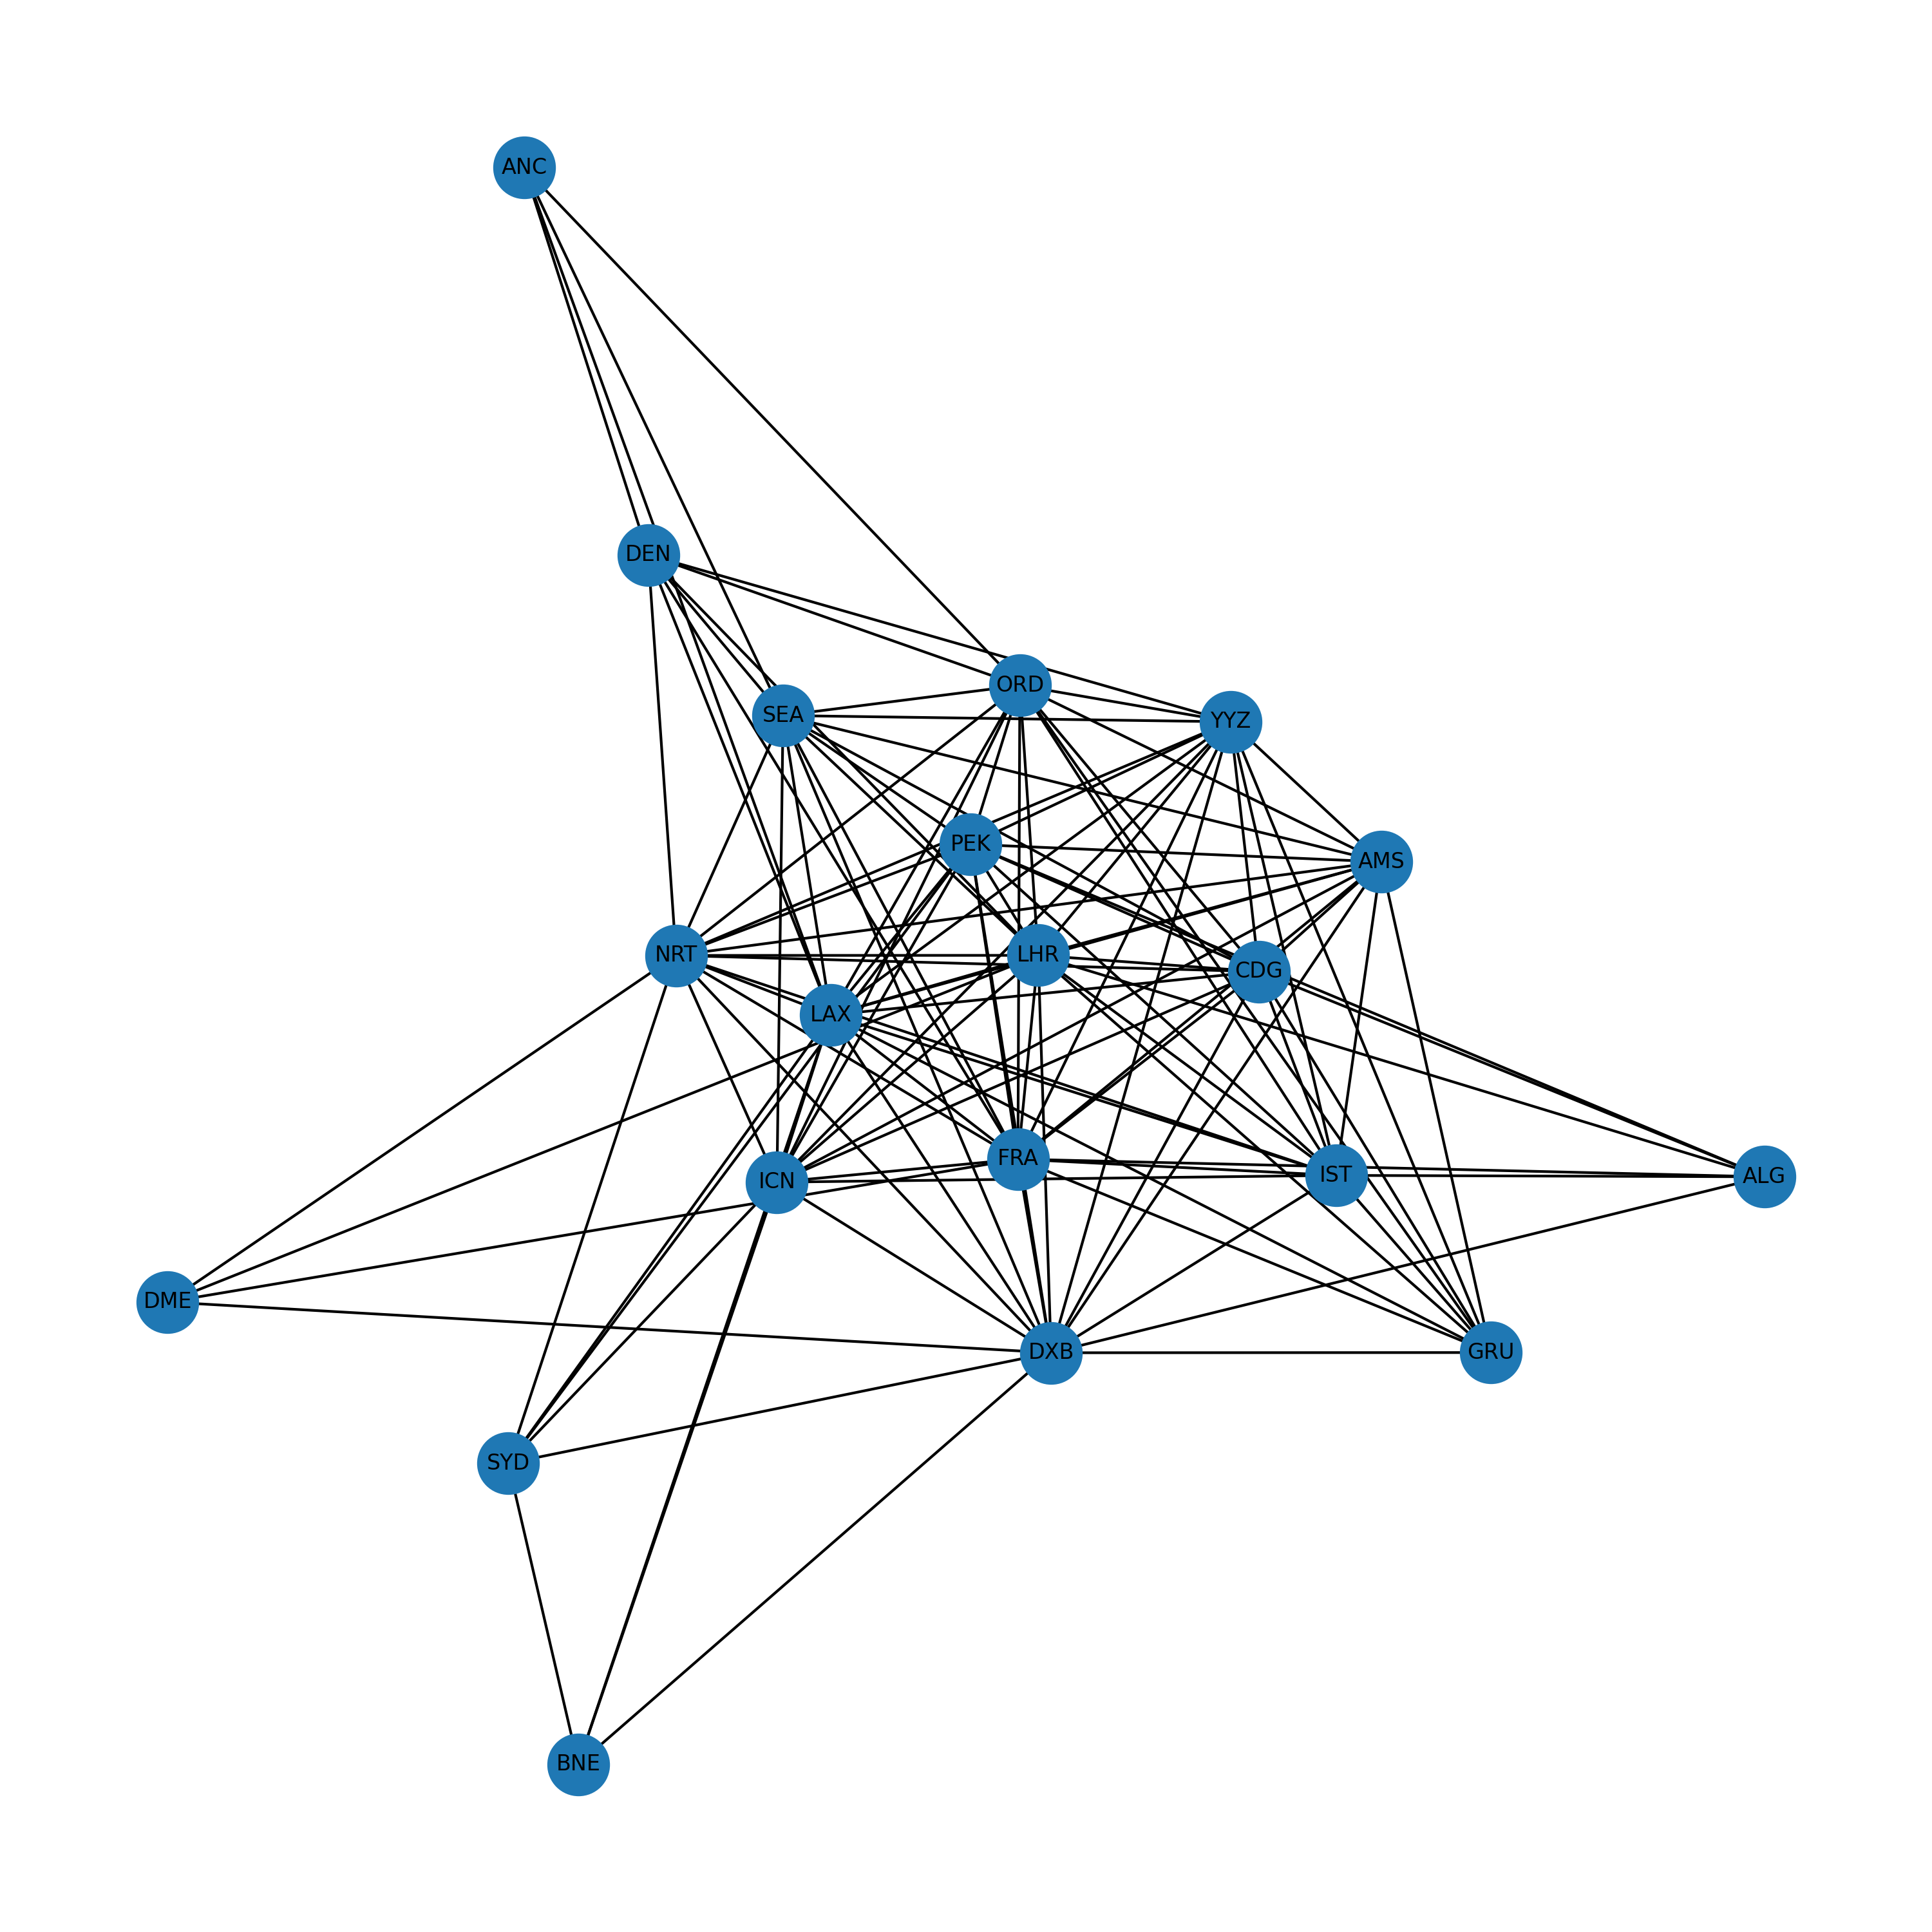
\includegraphics[width=0.9\textwidth]{chapter5/immagini/top20_betweenness_subgraph.png}
\caption{Sottografo dei top 20 aeroporti per betweenness centrality.}
\label{fig:top20_betweenness_subgraph}
\end{figure}

La Figura~\ref{fig:top20_betweenness_subgraph} mostra che questi nodi formano una sottorete molto densa, nella quale compaiono sia grandi hub internazionali sia aeroporti che assumono una funzione di snodo strategico. La visualizzazione conferma quindi che i nodi con betweenness più elevata non sono isolati, ma si collocano in una porzione altamente connessa della rete globale.

\section{Closeness centrality}

La closeness centrality misura quanto un nodo sia mediamente vicino a tutti gli altri nodi della rete. In una rete di trasporto, un aeroporto con elevata closeness può essere interpretato come uno scalo da cui è possibile raggiungere il resto del sistema con un numero relativamente ridotto di passaggi.

\begin{figure}[H]
\centering
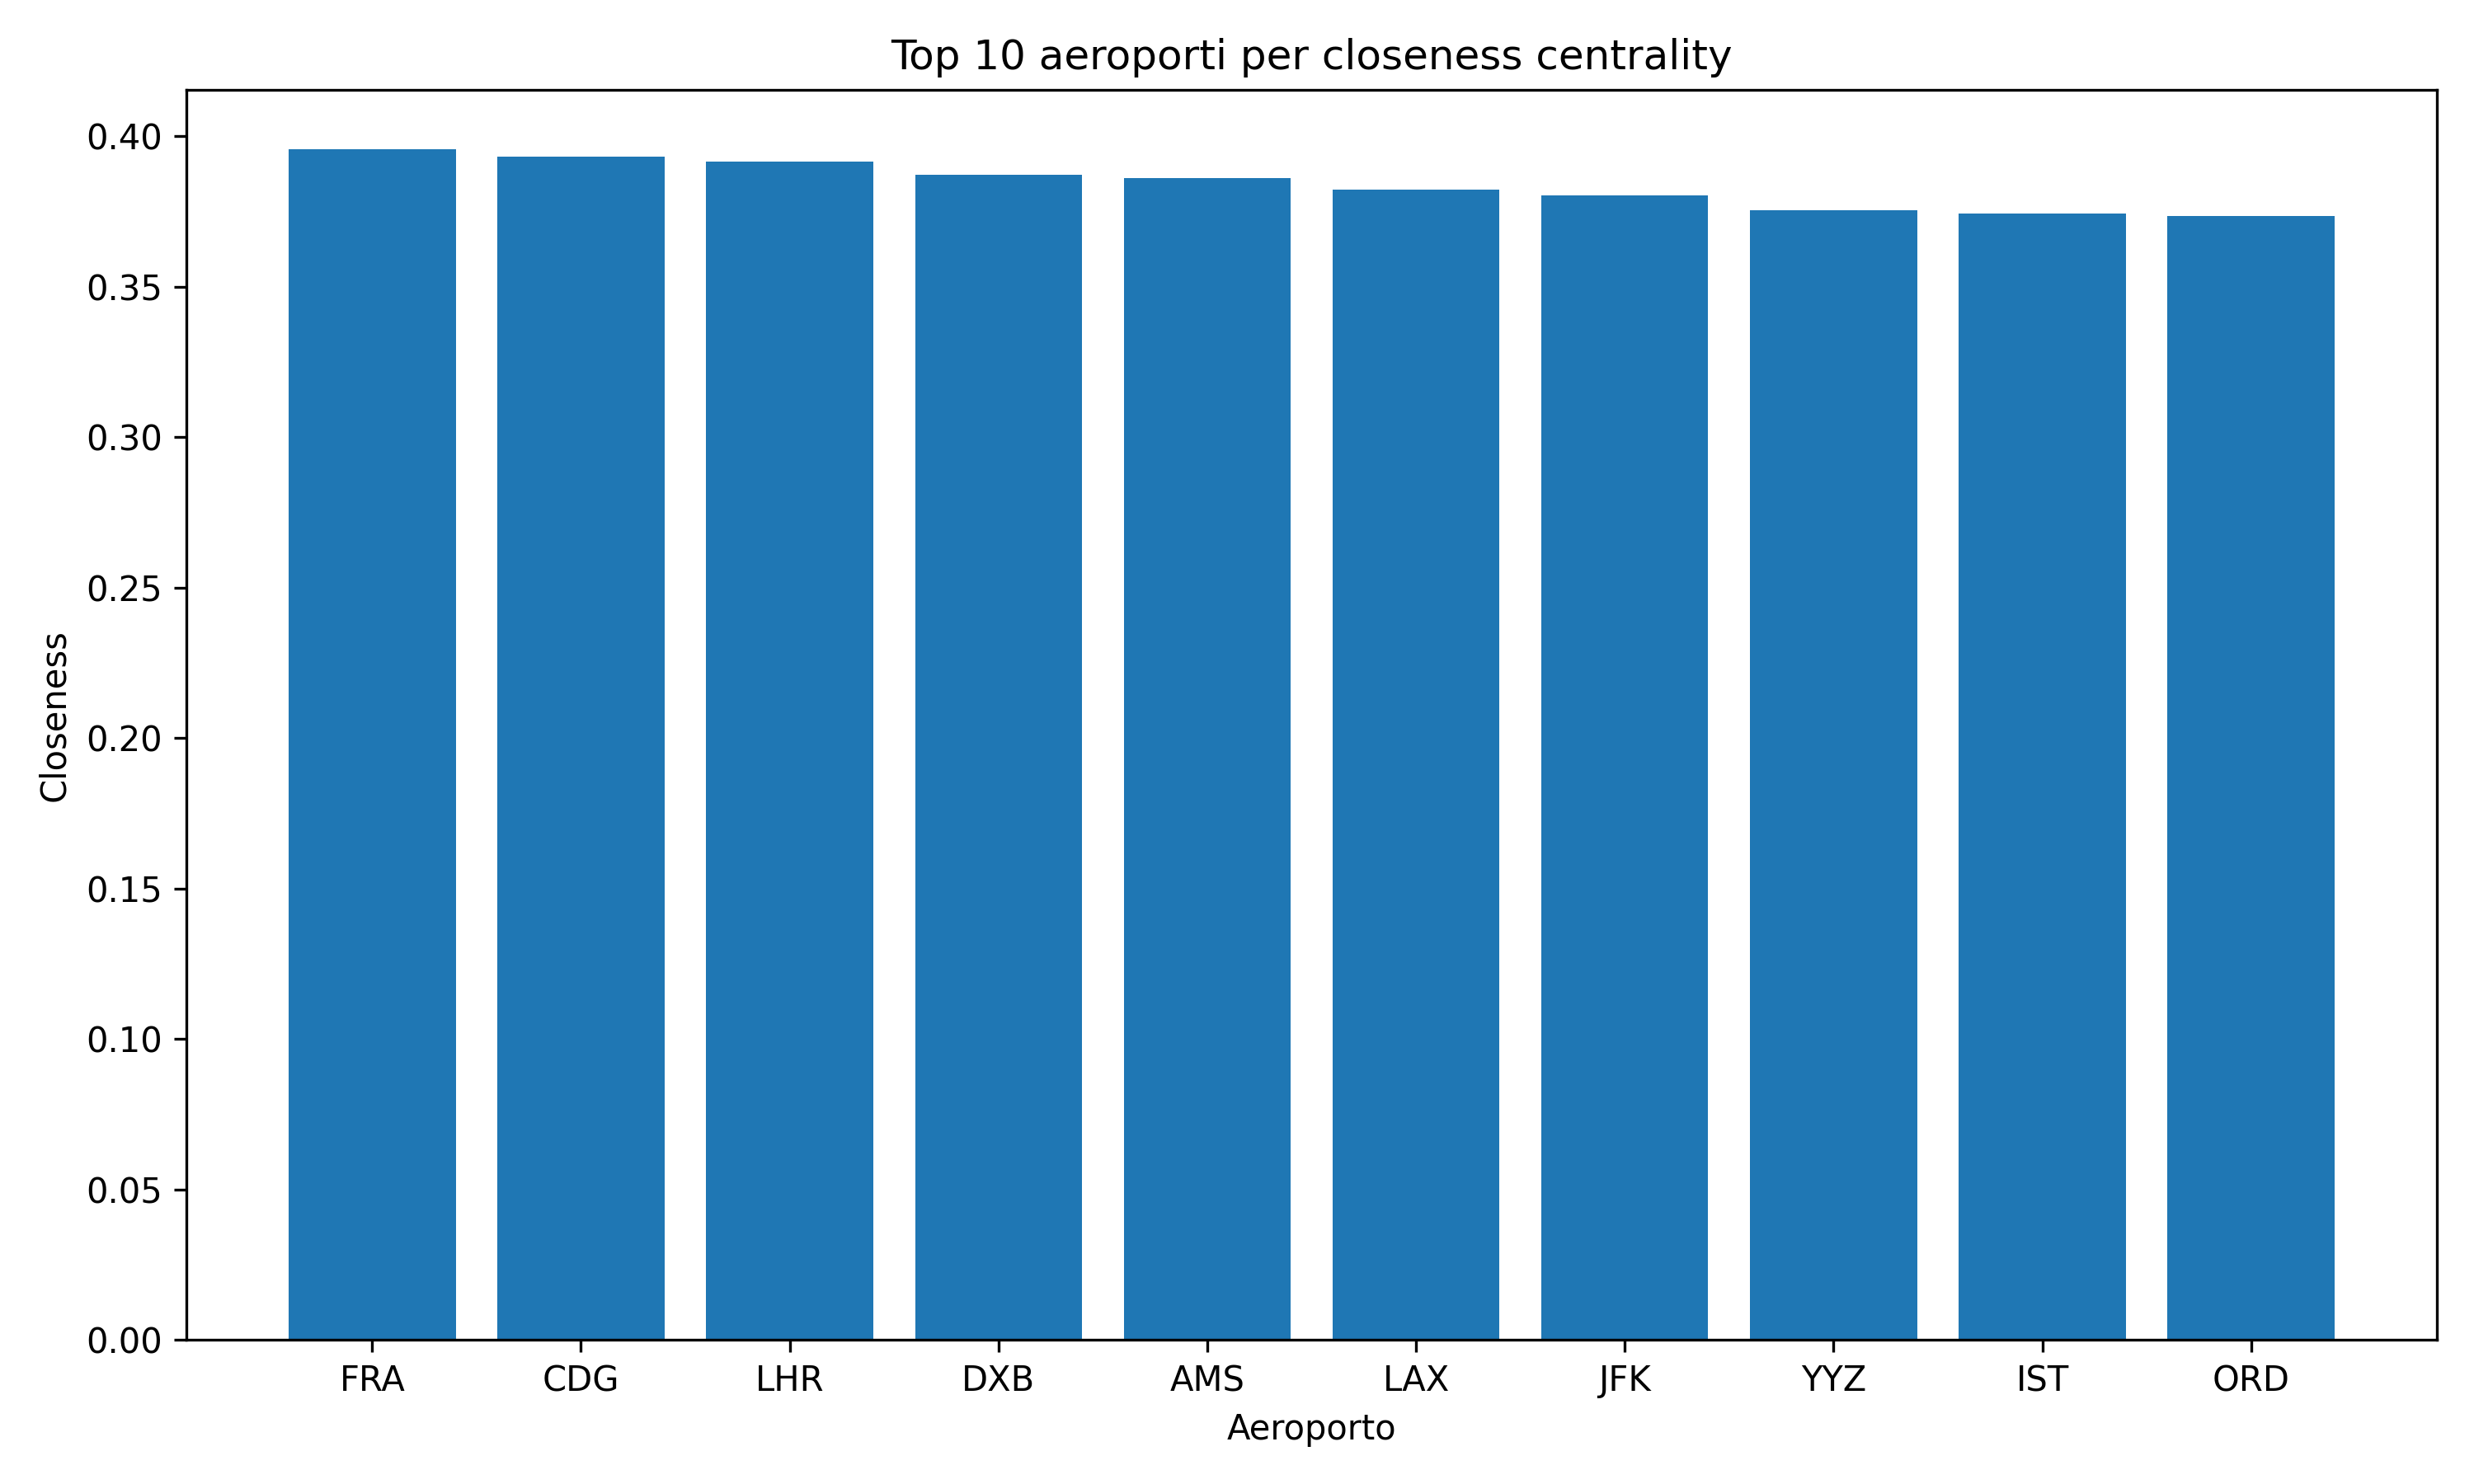
\includegraphics[width=0.9\textwidth]{chapter5/immagini/top10_closeness.png}
\caption{Top 10 aeroporti per closeness centrality.}
\label{fig:top_closeness}
\end{figure}

Dalla Figura~\ref{fig:top_closeness} emerge che gli aeroporti con i valori più alti di closeness sono FRA, CDG, LHR, DXB, AMS, LAX, JFK, YYZ, IST e ORD. In questo caso il ranking appare più vicino ai risultati ottenuti per degree, poiché gli aeroporti molto ben connessi tendono anche a risultare mediamente più vicini al resto della rete.

Il dato più evidente è la presenza di grandi hub internazionali europei, nordamericani e mediorientali, che appaiono strutturalmente ben posizionati per raggiungere un elevato numero di destinazioni con pochi passaggi intermedi. FRA, CDG e LHR si distinguono in particolare come nodi altamente accessibili all’interno del sistema complessivo.

Per completare questa osservazione, è stato costruito anche il sottografo dei 20 aeroporti con closeness centrality più elevata.

\begin{figure}[H]
\centering
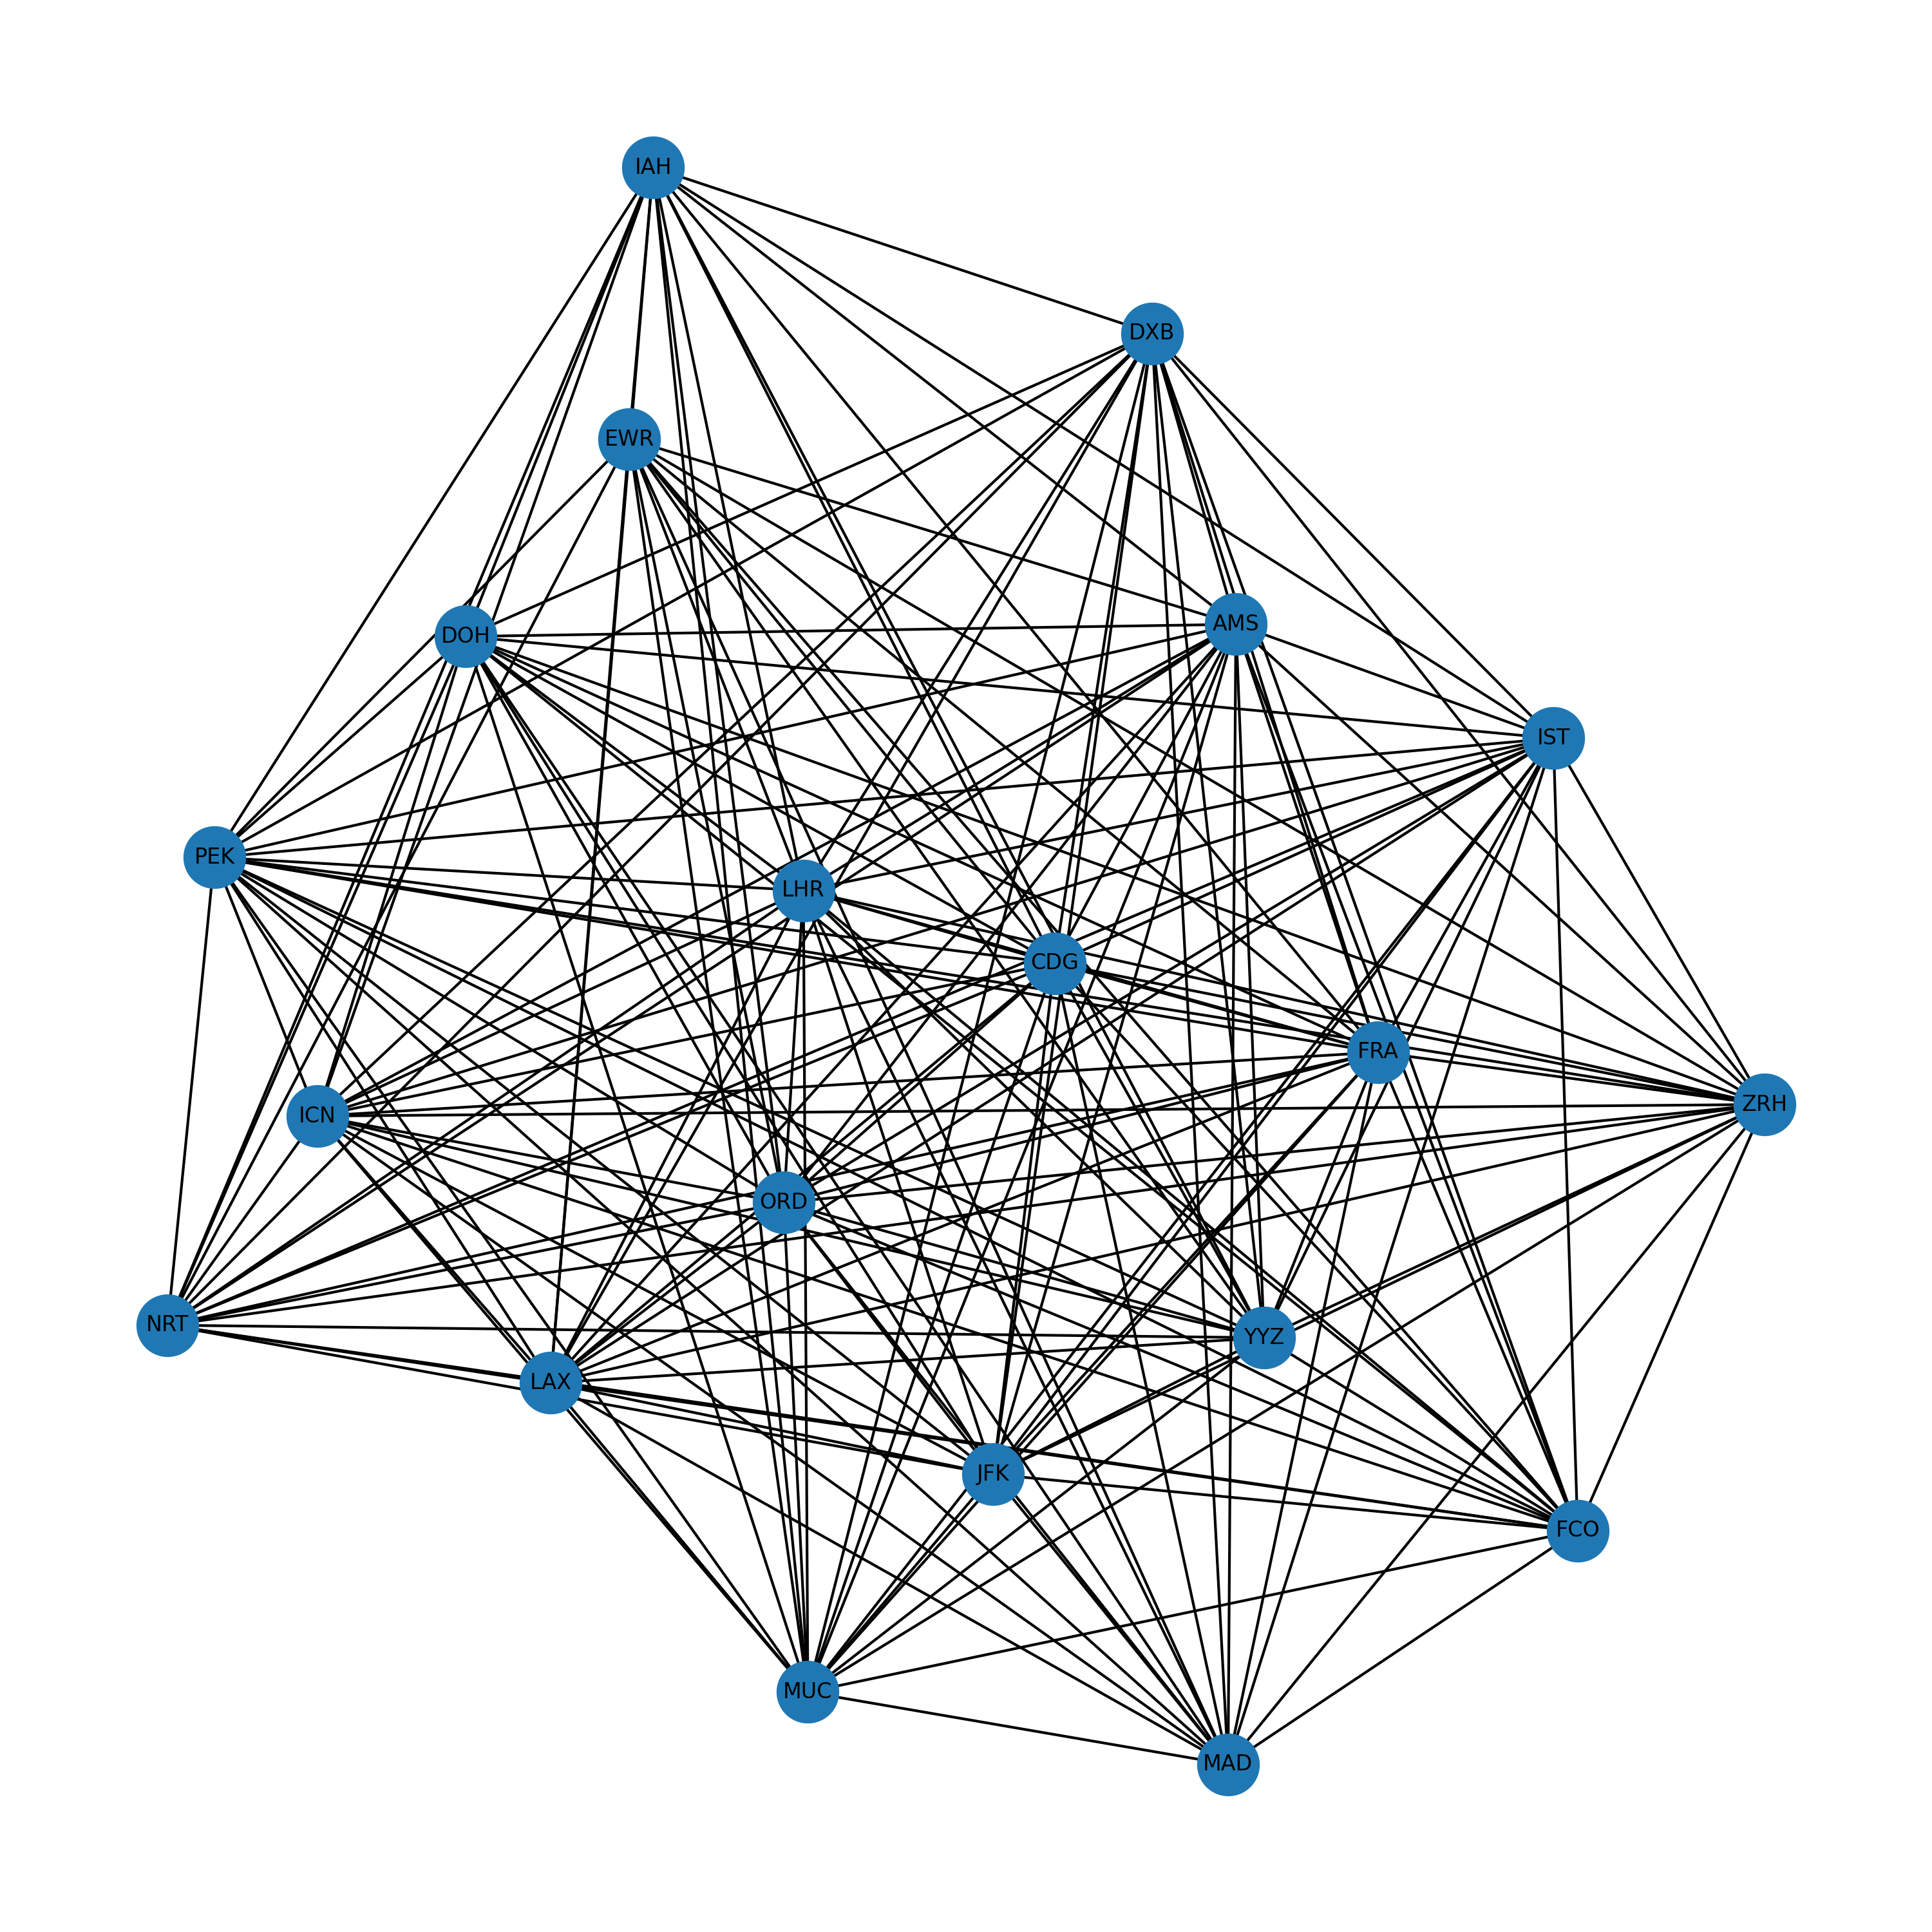
\includegraphics[width=0.9\textwidth]{chapter5/immagini/top20_closeness_subgraph.png}
\caption{Sottografo dei top 20 aeroporti per closeness centrality.}
\label{fig:top20_closeness_subgraph}
\end{figure}

La Figura~\ref{fig:top20_closeness_subgraph} evidenzia una sottorete molto compatta e fortemente interconnessa. Questo comportamento è coerente con il significato stesso della closeness: i nodi che risultano mediamente più vicini al resto della rete tendono anche a occupare posizioni centrali all’interno di una struttura molto fitta di collegamenti reciproci.

\section{PageRank}

Il PageRank rappresenta una misura di importanza che non considera soltanto il numero di collegamenti ricevuti, ma anche la rilevanza dei nodi da cui tali collegamenti provengono. Un aeroporto, dunque, assume un valore elevato se riceve molte connessioni, e se queste arrivano da nodi a loro volta importanti nella struttura della rete.

\begin{figure}[H]
\centering
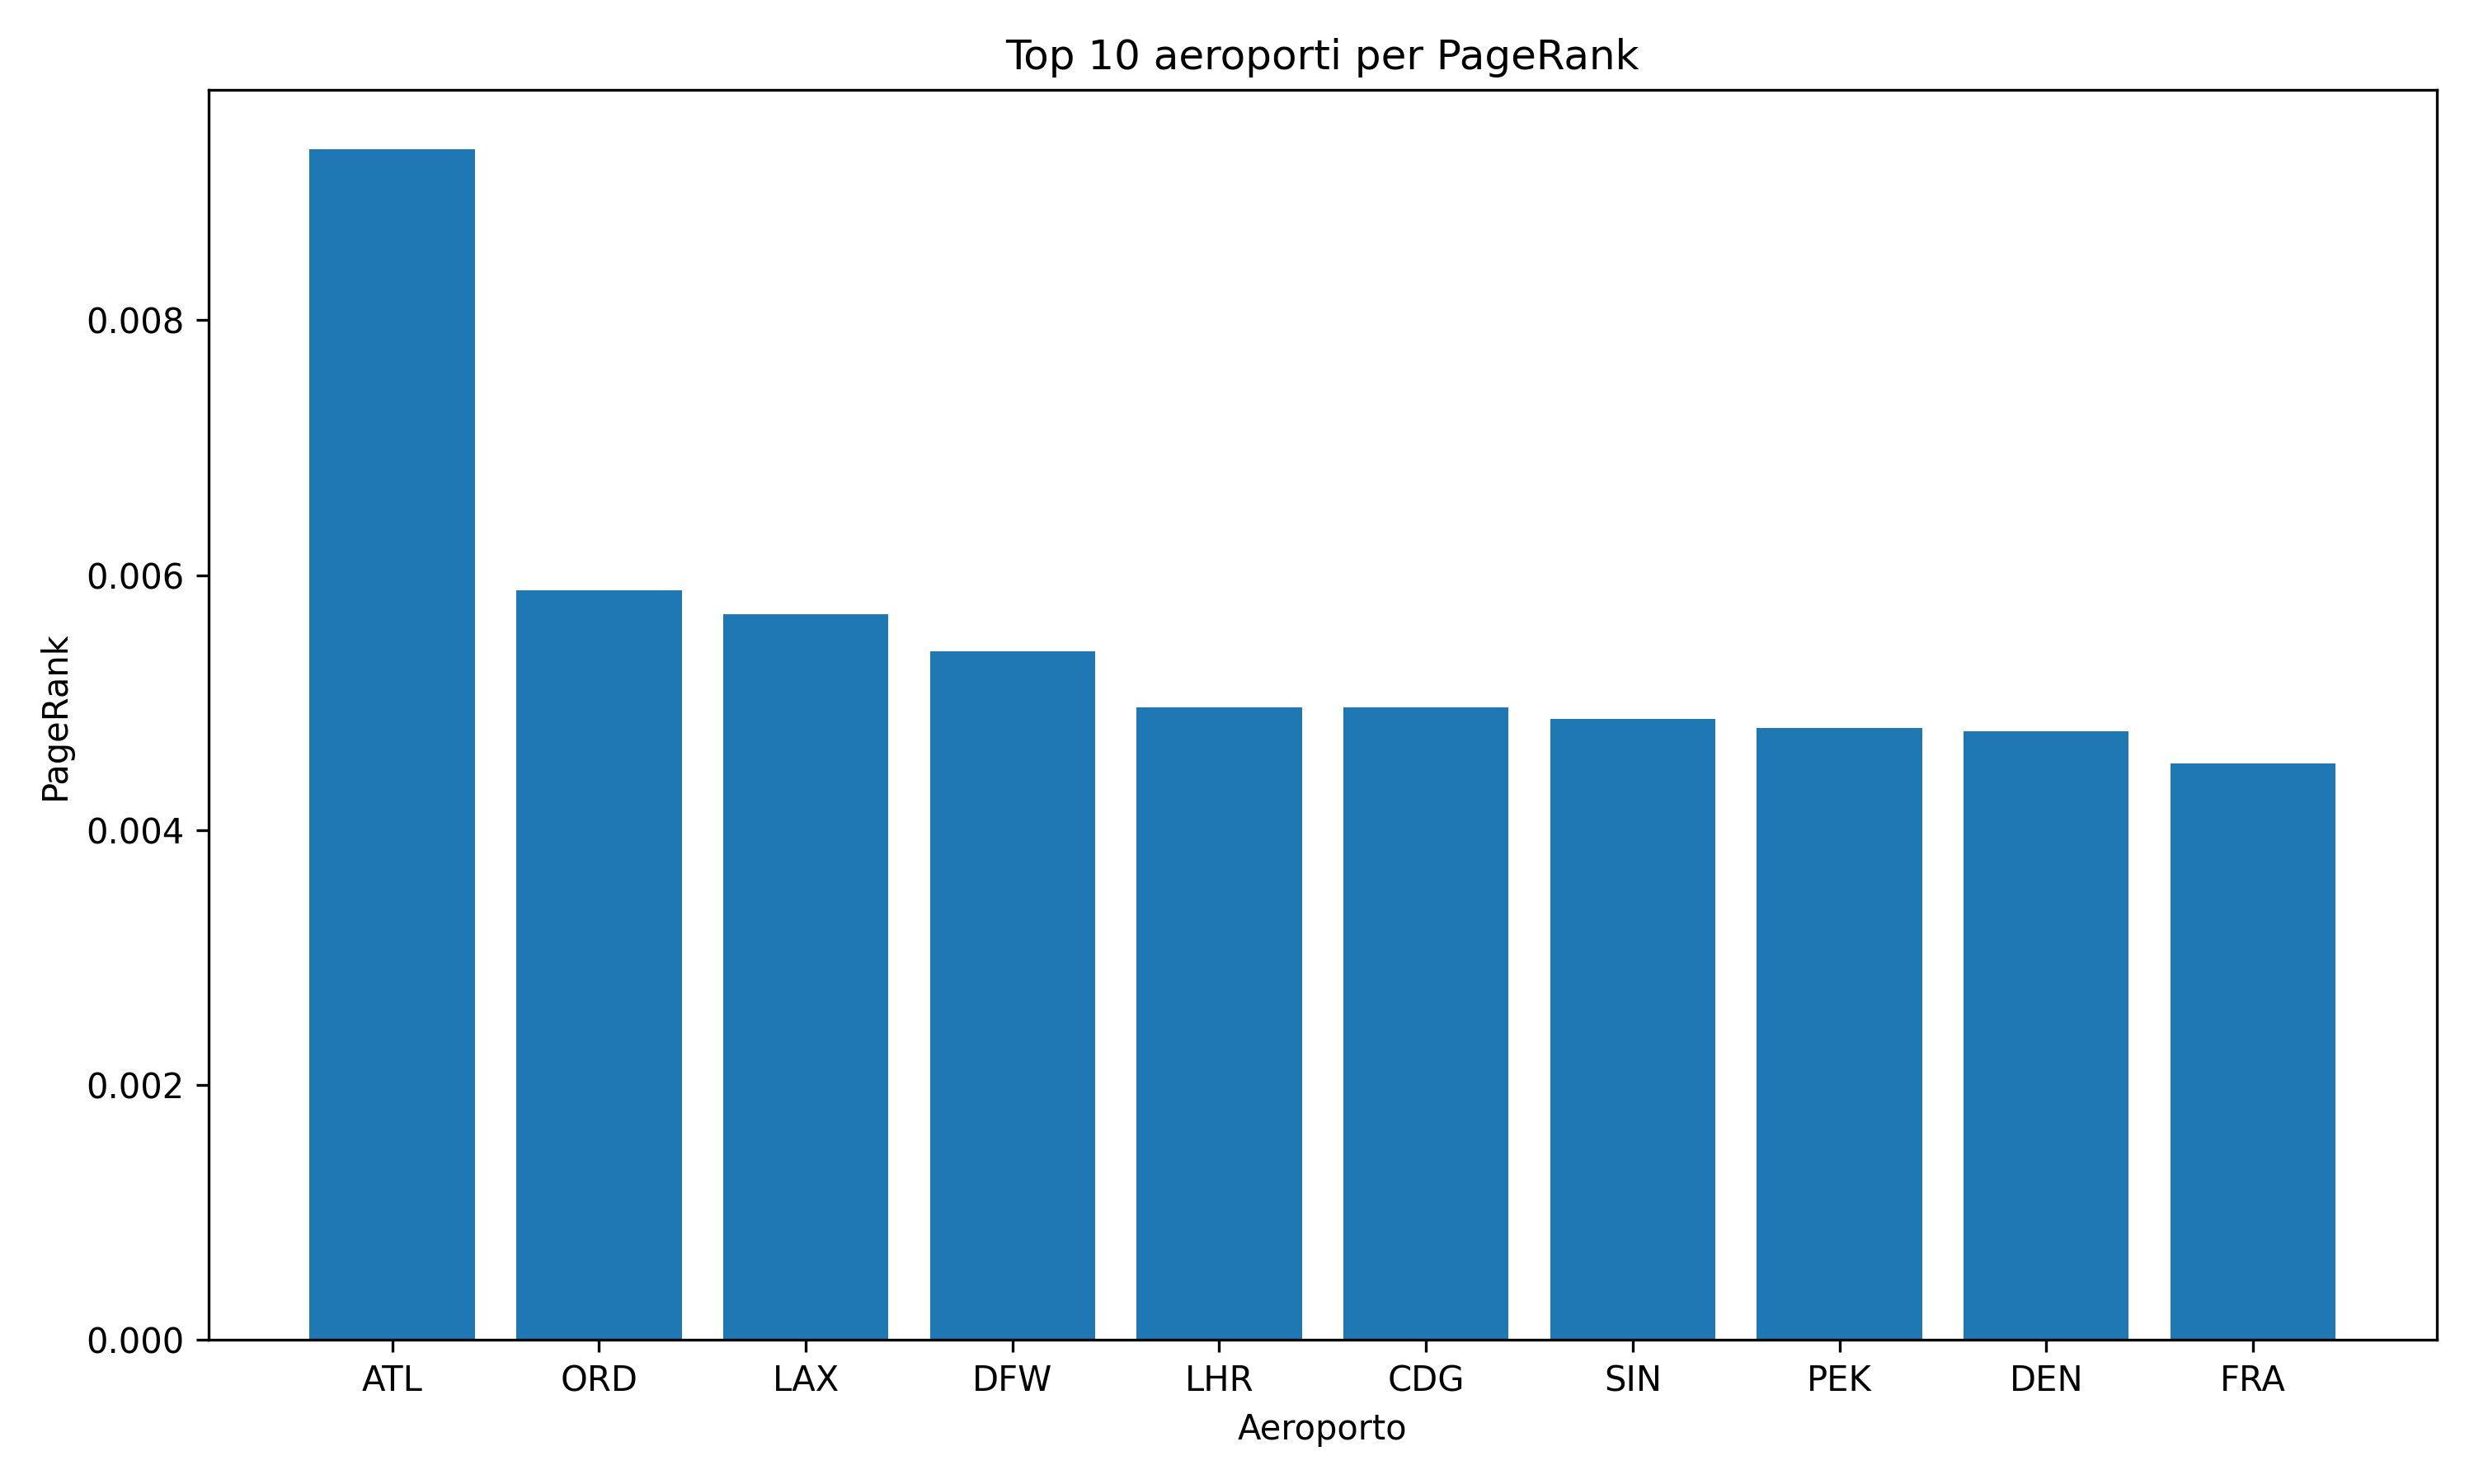
\includegraphics[width=0.9\textwidth]{chapter5/immagini/top10_pagerank.png}
\caption{Top 10 aeroporti per PageRank.}
\label{fig:top_pagerank}
\end{figure}

La Figura~\ref{fig:top_pagerank} mostra che gli aeroporti con più alto PageRank sono ATL, ORD, LAX, DFW, LHR, CDG, SIN, PEK, DEN e FRA. A differenza delle altre misure, qui emerge con particolare forza ATL, che occupa il primo posto con un valore sensibilmente più alto rispetto agli altri aeroporti.

Questo risultato indica che ATL non è soltanto un nodo molto connesso, ma anche uno scalo inserito in una parte strutturalmente molto rilevante della rete. In generale, il PageRank tende a valorizzare aeroporti fortemente integrati nei flussi principali del sistema, premiando la qualità delle connessioni più che la sola quantità.

Anche in questo caso è stato generato il sottografo dei primi 20 aeroporti per PageRank.

\begin{figure}[H]
\centering
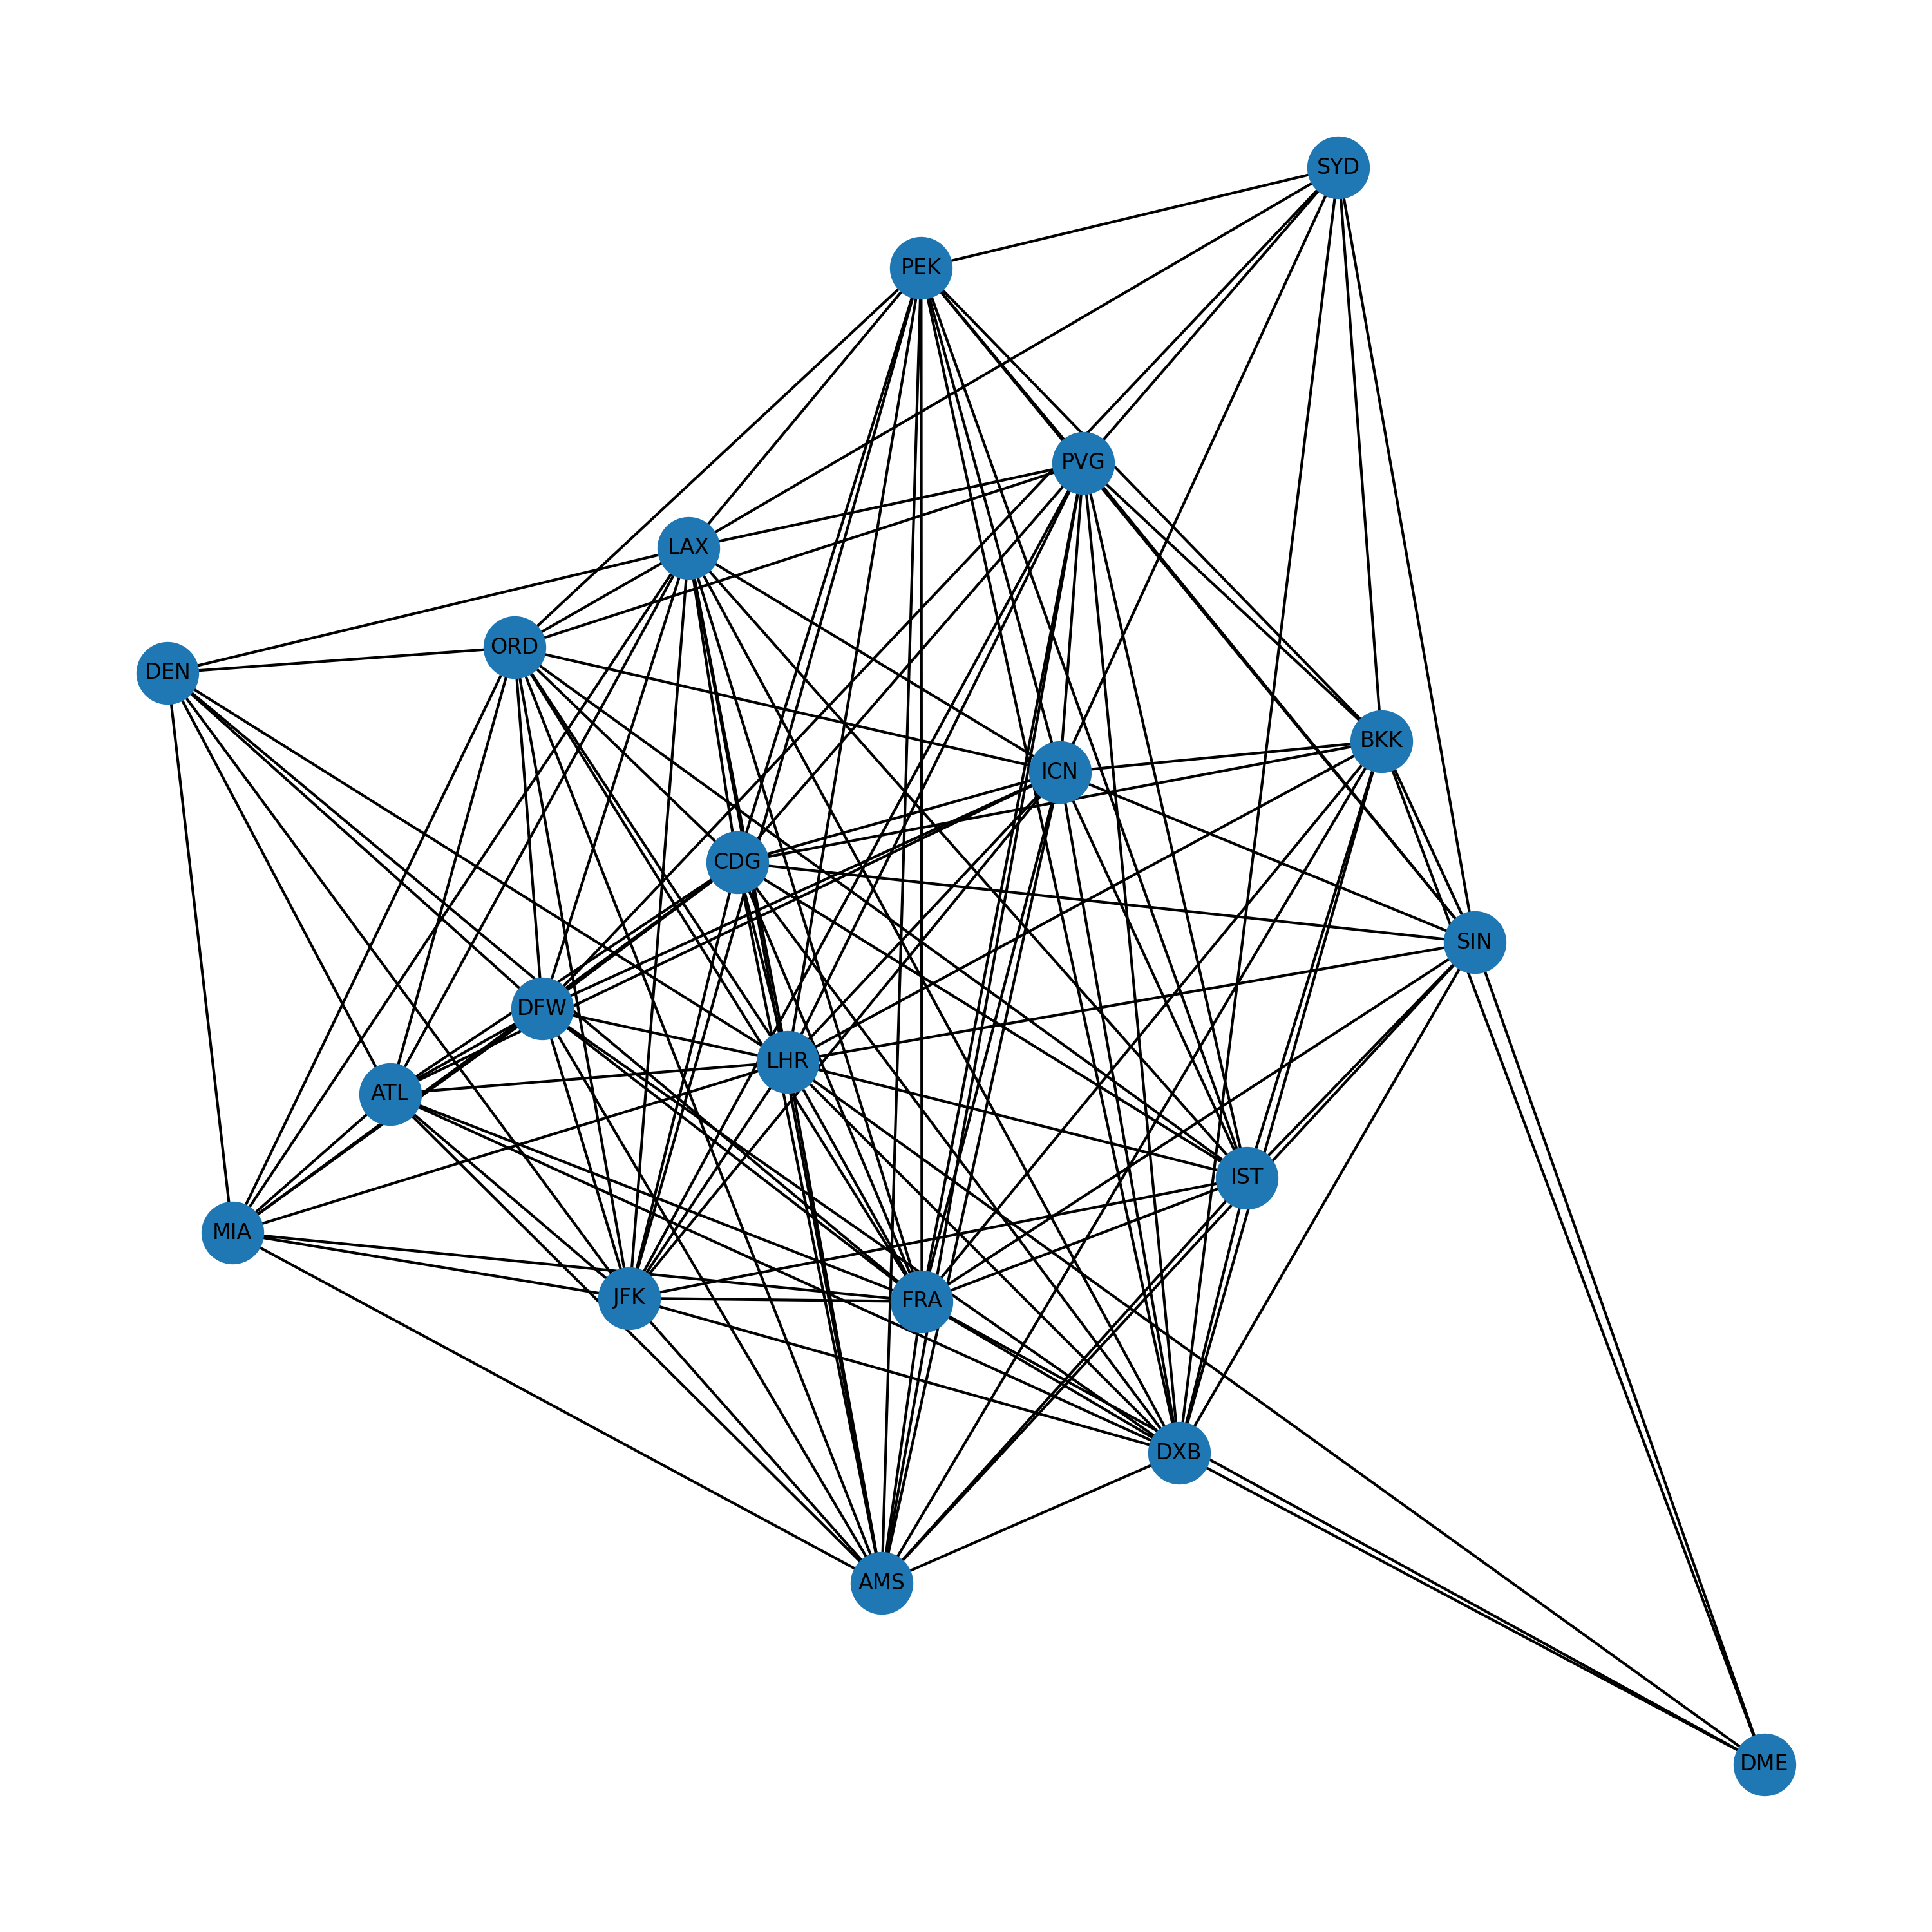
\includegraphics[width=0.9\textwidth]{chapter5/immagini/top20_pagerank_subgraph.png}
\caption{Sottografo dei top 20 aeroporti per PageRank.}
\label{fig:top20_pagerank_subgraph}
\end{figure}

Come mostrato nella Figura~\ref{fig:top20_pagerank_subgraph}, i nodi con più alto PageRank formano anch’essi una sottorete fortemente connessa. In questo caso, la struttura appare particolarmente interessante perché mette in evidenza un insieme di hub globali non solo ben collegati, ma anche fortemente inseriti nelle connessioni più influenti della rete.

\section{Eigenvector centrality}

L’eigenvector centrality misura l’importanza di un nodo tenendo conto non solo del numero di collegamenti, ma anche della centralità dei nodi a cui esso è connesso. Un aeroporto, dunque, assume un valore elevato se è collegato ad altri aeroporti che risultano a loro volta particolarmente centrali nella struttura della rete.

Nel presente progetto questa misura è stata calcolata sulla versione non diretta della largest weakly connected component, che contiene 3397 nodi e 37547 archi. Tale scelta consente di ottenere una rappresentazione più stabile e interpretabile del prestigio strutturale dei nodi all’interno del sistema complessivo.

\begin{figure}[H]
\centering
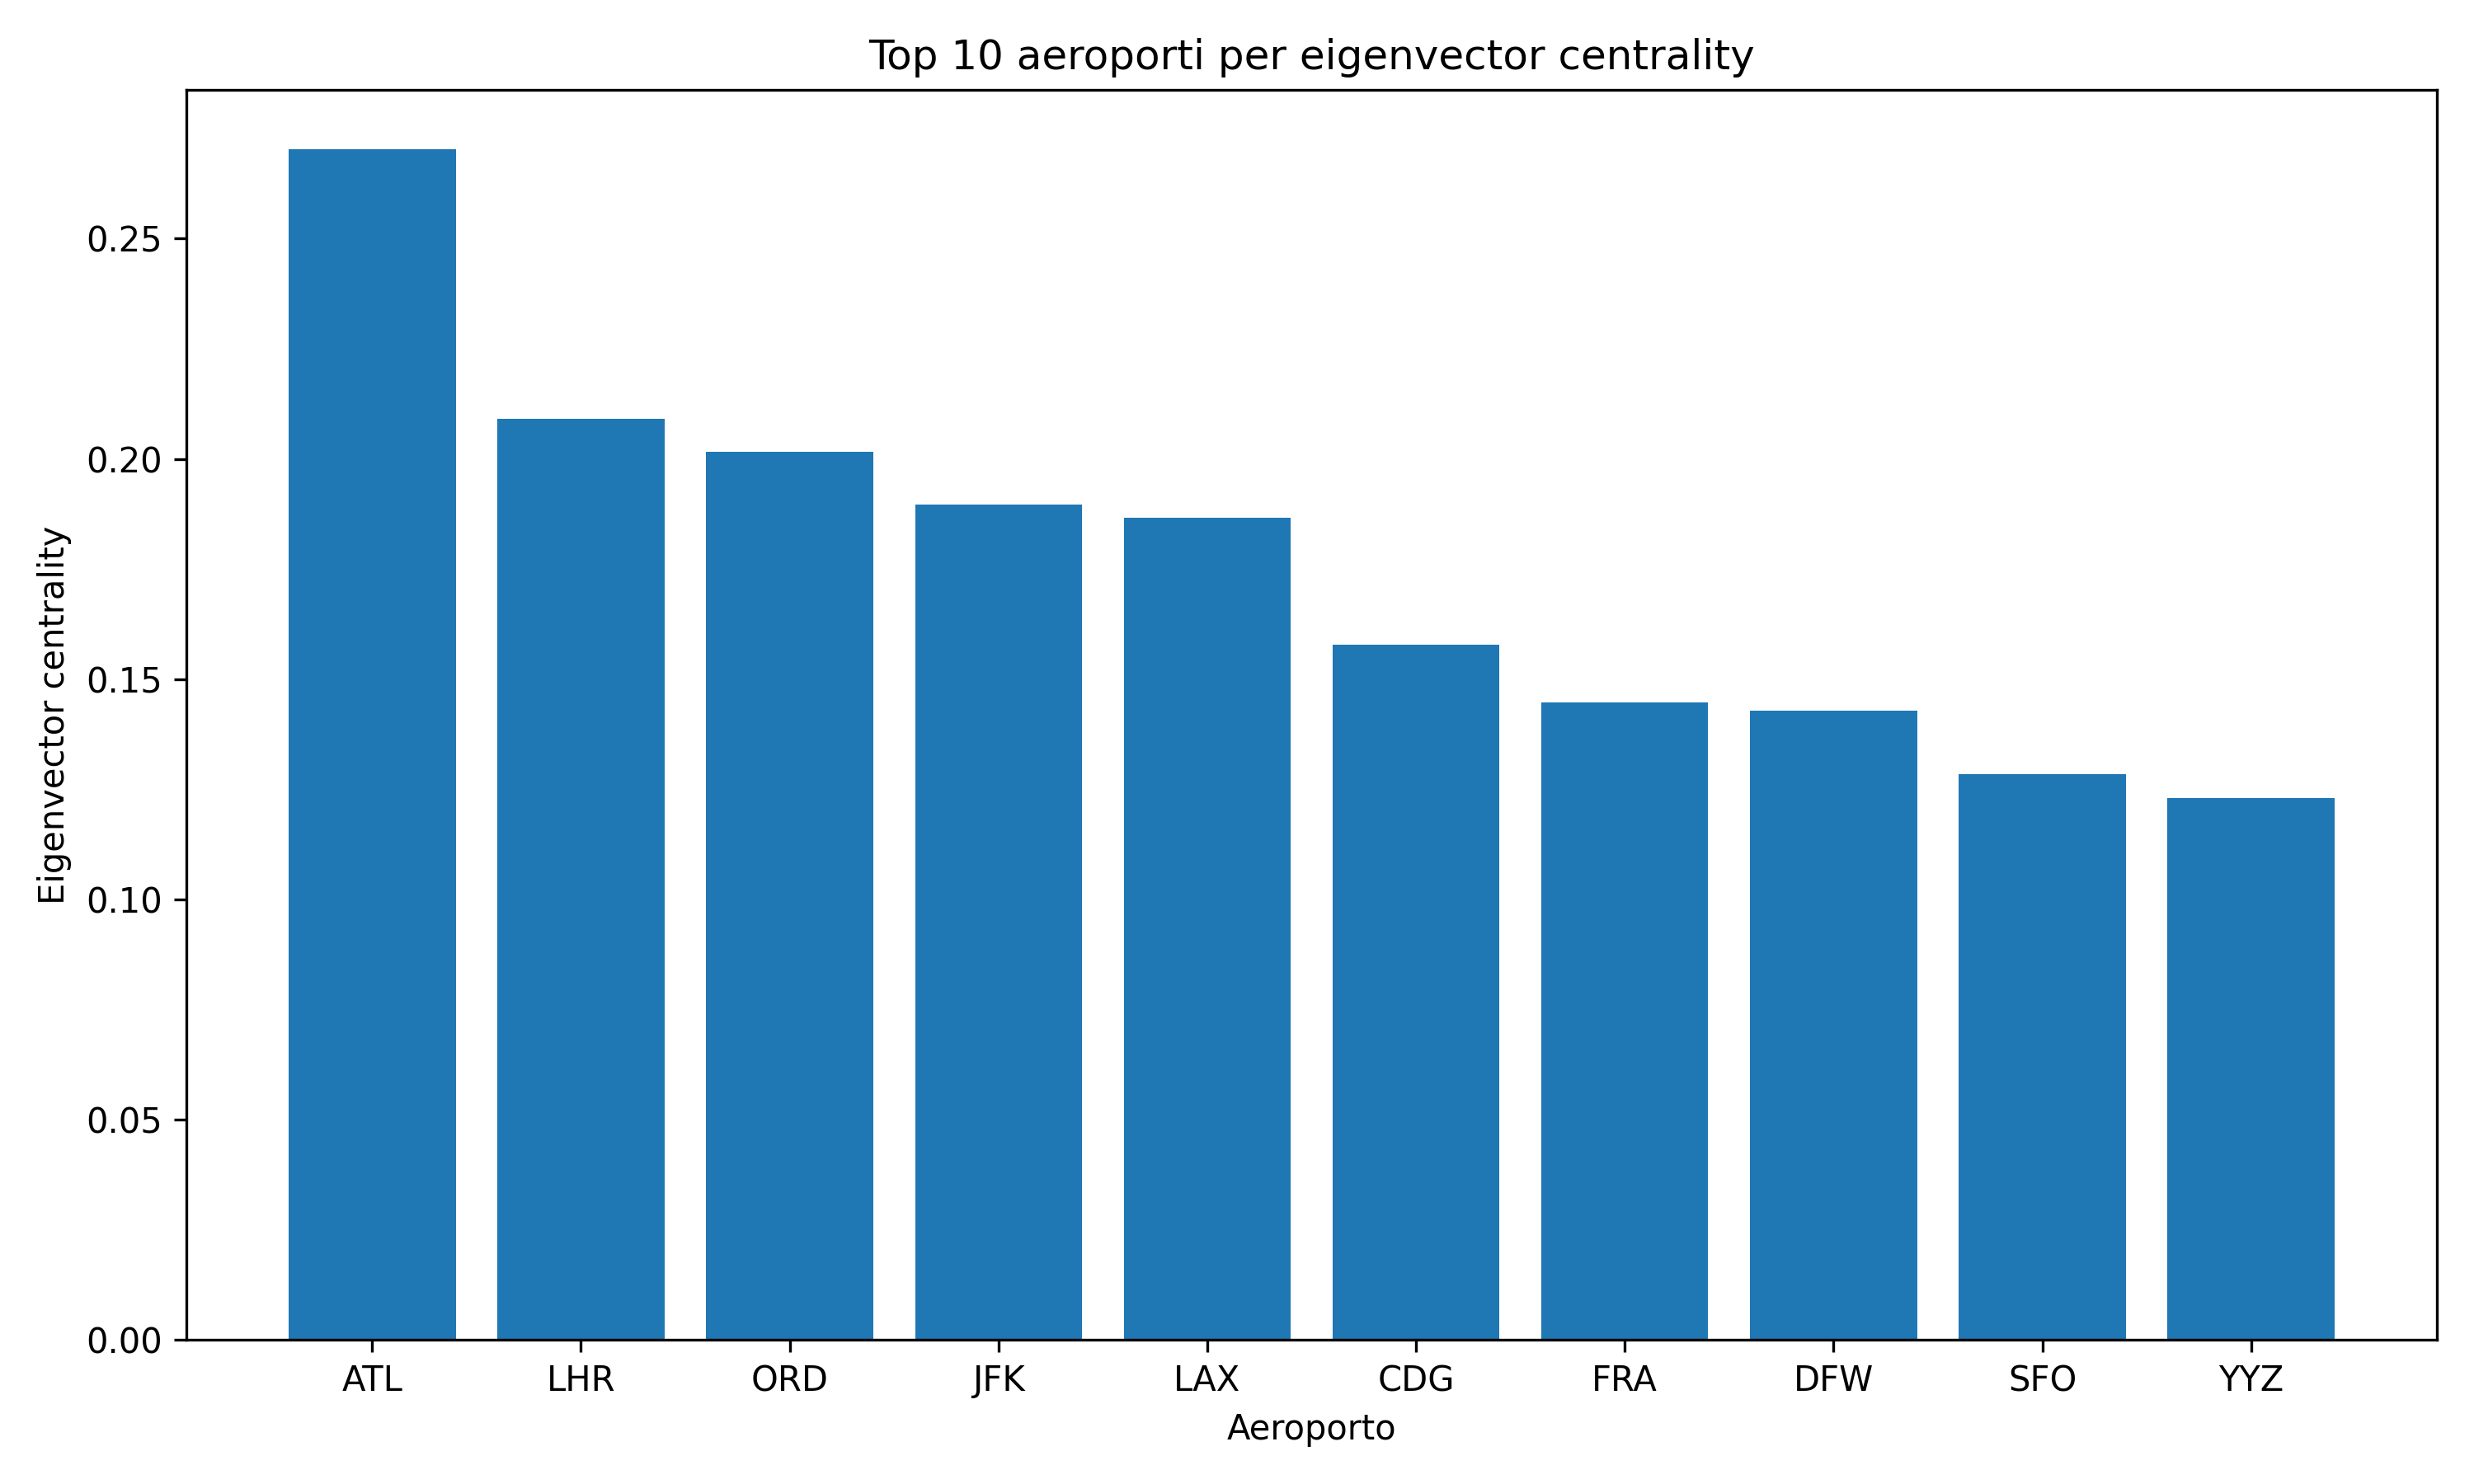
\includegraphics[width=0.9\textwidth]{chapter5/immagini/top10_eigenvector.png}
\caption{Top 10 aeroporti per eigenvector centrality.}
\label{fig:top_eigenvector}
\end{figure}

La Figura~\ref{fig:top_eigenvector} mostra che gli aeroporti con i valori più elevati di eigenvector centrality sono ATL, LHR, ORD, JFK, LAX, CDG, FRA, DFW, SFO e YYZ. Il risultato è particolarmente interessante perché evidenzia un nucleo di hub fortemente inseriti nelle porzioni più centrali e influenti della rete.

A differenza della betweenness centrality, che premia i nodi con forte capacità di intermediazione, l’eigenvector centrality tende a valorizzare aeroporti che appartengono al nucleo strutturalmente più prestigioso del sistema. In questo senso, il primo posto di ATL suggerisce che tale aeroporto non sia solo molto connesso, ma anche profondamente integrato in una parte della rete formata da nodi a loro volta altamente centrali.

Per osservare meglio le relazioni tra i principali aeroporti secondo questa misura, è stato costruito anche il sottografo dei primi 20 nodi per eigenvector centrality.

\begin{figure}[H]
\centering
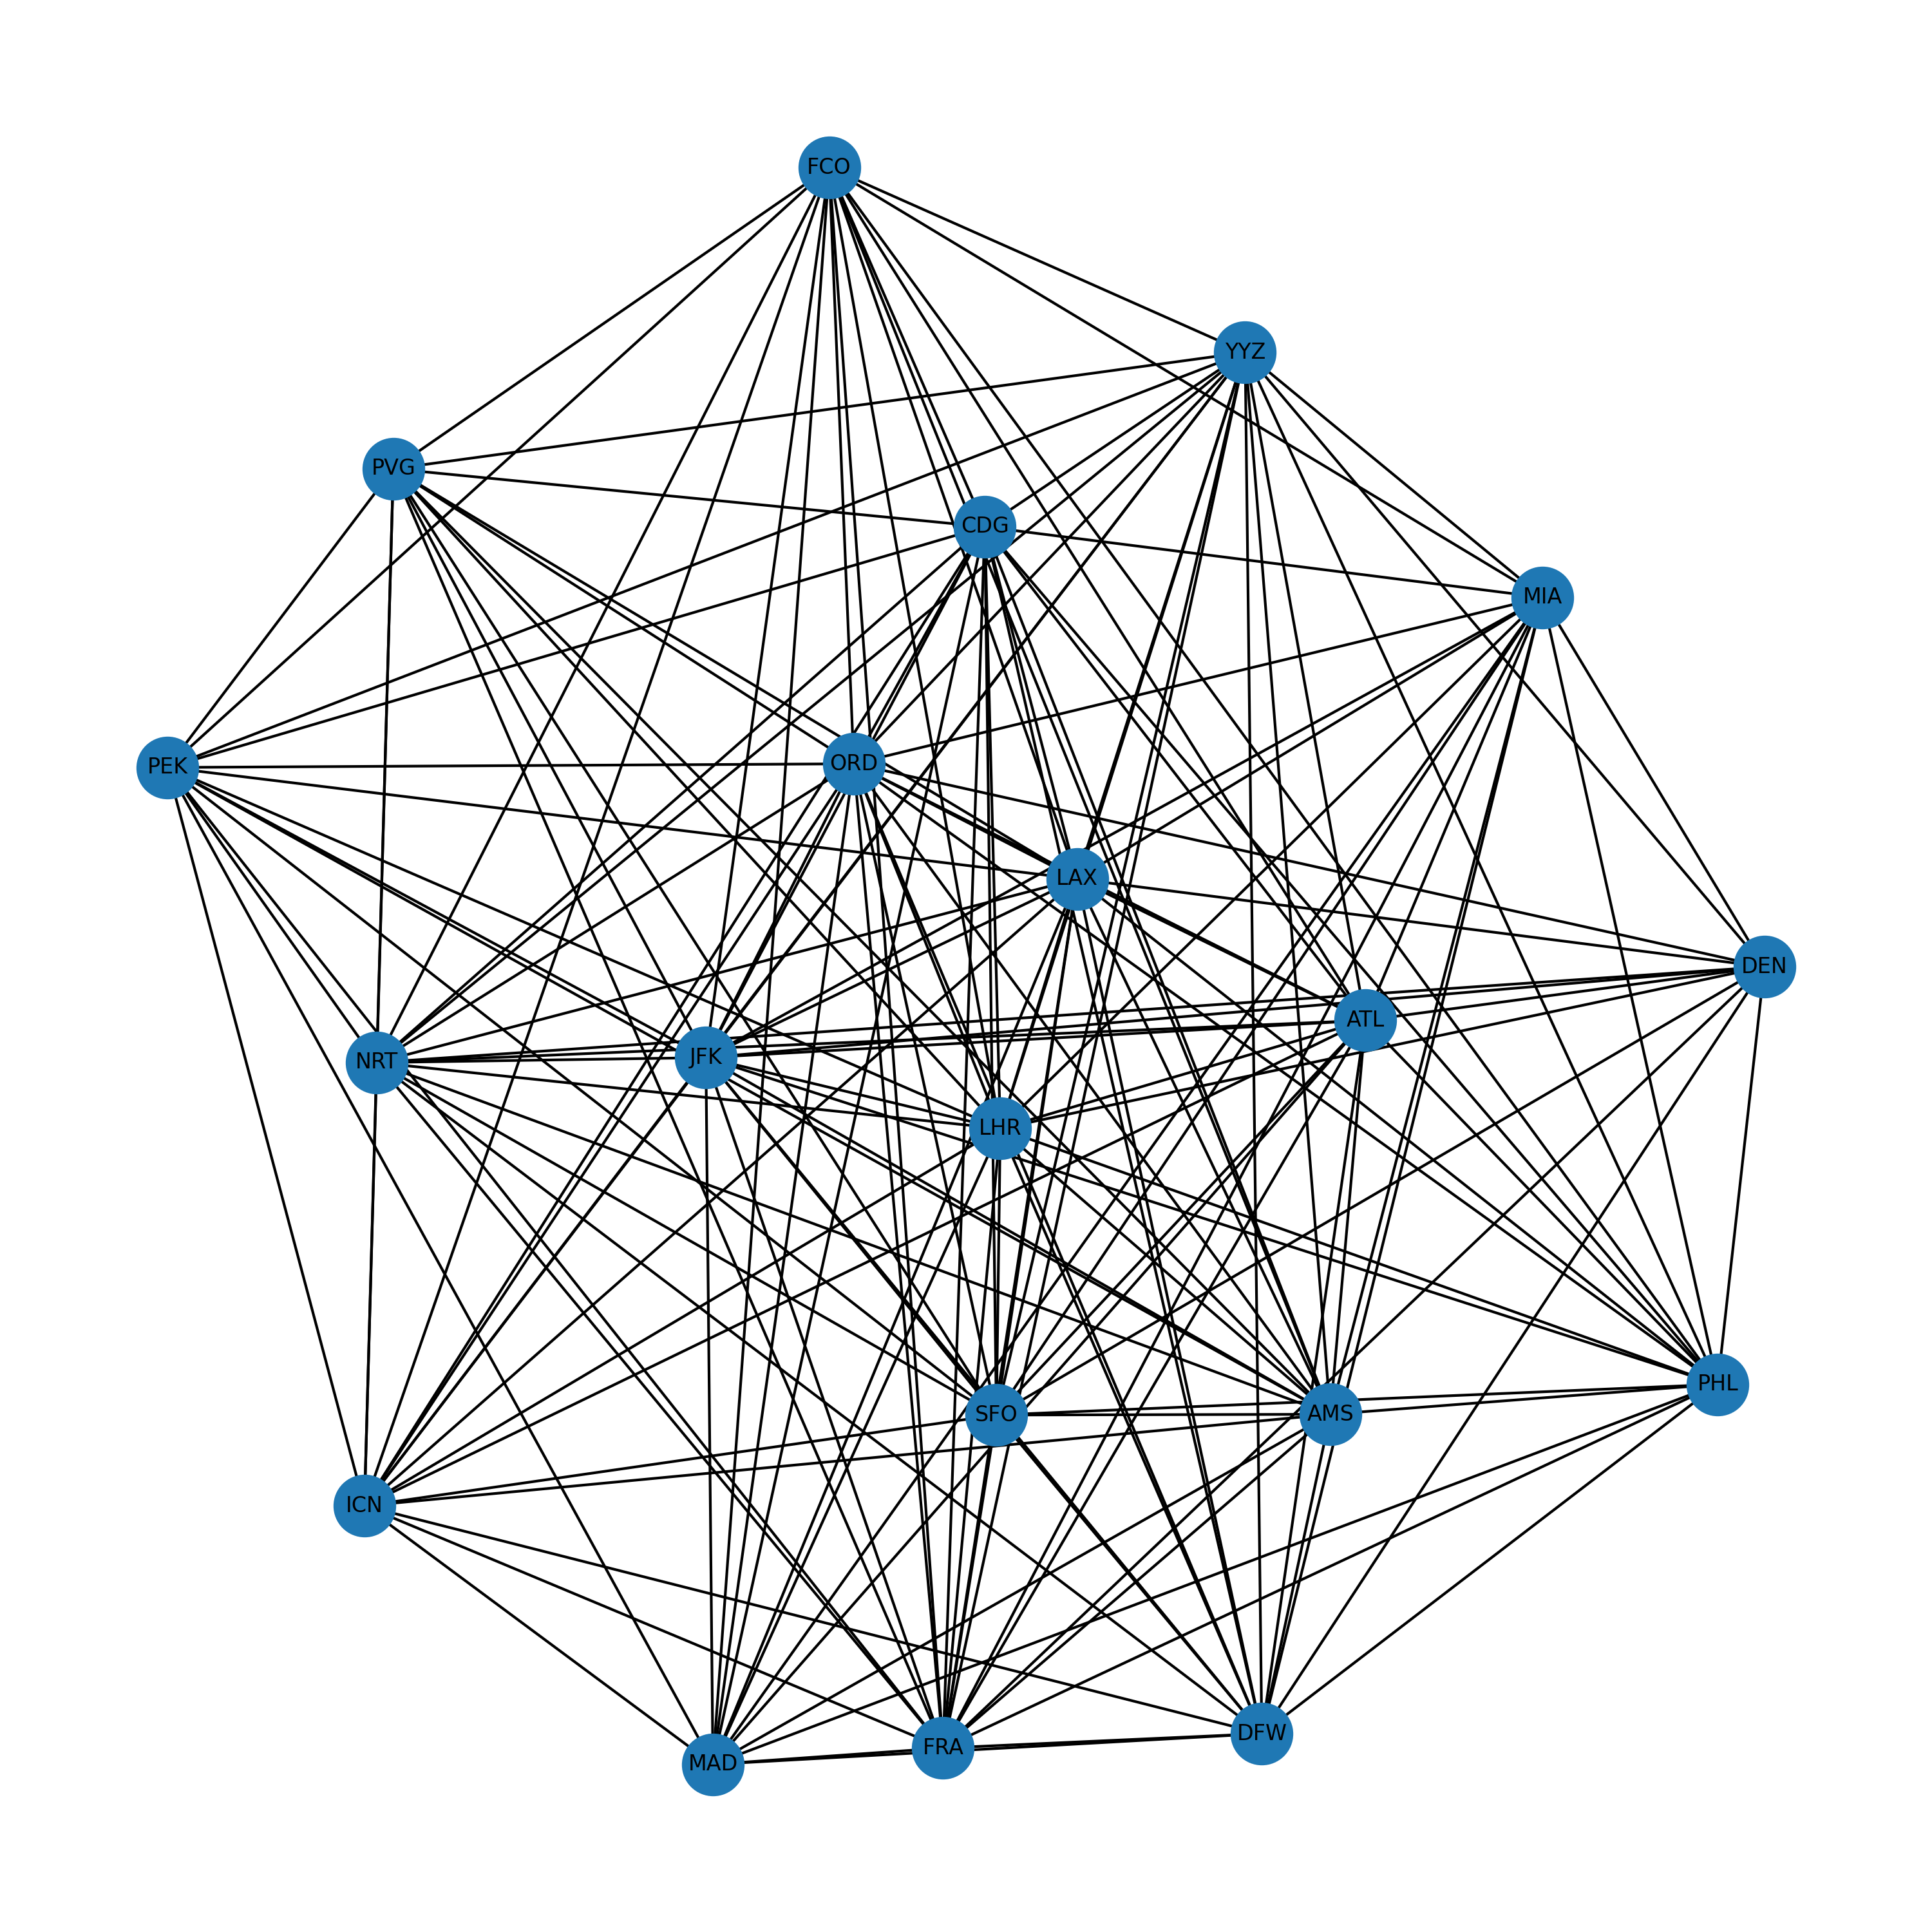
\includegraphics[width=0.9\textwidth]{chapter5/immagini/top20_eigenvector_subgraph.png}
\caption{Sottografo dei top 20 aeroporti per eigenvector centrality.}
\label{fig:top20_eigenvector_subgraph}
\end{figure}

La Figura~\ref{fig:top20_eigenvector_subgraph} evidenzia una sottorete particolarmente densa, coerente con il significato della misura: gli aeroporti che emergono secondo l’eigenvector centrality tendono a occupare posizioni centrali all’interno del nucleo più influente della rete. La forte interconnessione tra questi nodi conferma che tale misura seleziona soprattutto aeroporti immersi nella parte più compatta e strategica del sistema.

\section{Confronto tra le misure di centralità}

Le quattro misure considerate mettono in luce aspetti differenti della rilevanza strutturale dei nodi. In particolare, la betweenness centrality evidenzia aeroporti che fungono da ponti strategici tra zone diverse della rete, la closeness centrality mette in risalto gli aeroporti più accessibili rispetto al resto del sistema, il PageRank individua nodi strutturalmente importanti in base al prestigio dei collegamenti ricevuti, mentre l’eigenvector centrality valorizza gli aeroporti connessi al nucleo più centrale e influente della rete.

Per confrontare in modo sintetico i risultati ottenuti sulle principali misure di centralità calcolate sul grafo diretto, è stata costruita la Tabella~\ref{tab:centrality_comparison}, che riporta l’unione dei nodi presenti nei top 10 di betweenness centrality, closeness centrality e PageRank. L’eigenvector centrality viene invece discussa separatamente, poiché è stata calcolata sulla versione non diretta della largest weakly connected component e mette in evidenza in modo particolare il nucleo più prestigioso della rete.

\begin{table}[H]
\centering
\caption{Confronto tra i nodi presenti nei top 10 delle principali misure di centralità. I valori assenti indicano che l’aeroporto non compare tra i primi dieci della misura considerata.}
\label{tab:centrality_comparison}
\begin{tabular}{lccc}
\toprule
\textbf{Aeroporto} & \textbf{Betweenness} & \textbf{Closeness} & \textbf{PageRank} \\
\midrule
AMS & -- & 0.386090 & -- \\
ANC & 0.062190 & -- & -- \\
ATL & -- & -- & 0.009340 \\
CDG & 0.057353 & 0.393208 & 0.004959 \\
DEN & -- & -- & 0.004777 \\
DFW & -- & -- & 0.005401 \\
DXB & 0.069143 & 0.387251 & -- \\
FRA & 0.054810 & 0.395624 & 0.004526 \\
IST & -- & 0.374432 & -- \\
JFK & -- & 0.380387 & -- \\
LAX & 0.069159 & 0.382168 & 0.005695 \\
LHR & 0.046764 & 0.391507 & 0.004960 \\
ORD & 0.043574 & 0.373430 & 0.005882 \\
PEK & 0.054857 & -- & 0.004800 \\
SEA & 0.071821 & -- & -- \\
SIN & -- & -- & 0.004869 \\
YYZ & 0.047524 & 0.375482 & -- \\
\bottomrule
\end{tabular}
\end{table}

La tabella mette in evidenza che alcuni aeroporti, come CDG, FRA, LAX, LHR e ORD, compaiono in più ranking, suggerendo una rilevanza strutturale multidimensionale. Altri nodi, invece, risultano particolarmente importanti solo rispetto a una specifica misura: è il caso di SEA e ANC per la betweenness, oppure di ATL e SIN nel ranking PageRank. Questo conferma che le diverse centralità non sono ridondanti, ma colgono aspetti complementari del ruolo dei nodi nella rete. L’eigenvector centrality rafforza ulteriormente questa osservazione, mettendo in evidenza gli aeroporti più fortemente inseriti nel nucleo centrale e influente del sistema.

Per sintetizzare il significato delle misure utilizzate, si può fare riferimento alla Tabella~\ref{tab:centrality_meaning}.

\begin{table}[H]
\centering
\caption{Interpretazione delle misure di centralità considerate nel progetto.}
\label{tab:centrality_meaning}
\begin{tabular}{ll}
\toprule
\textbf{Misura} & \textbf{Interpretazione principale} \\
\midrule
Betweenness centrality & Capacità del nodo di fungere da ponte nella rete \\
Closeness centrality & Vicinanza media del nodo al resto del sistema \\
PageRank & Importanza strutturale basata sulla qualità dei collegamenti ricevuti \\
Eigenvector centrality & Importanza del nodo in base alla centralità dei nodi vicini \\
\bottomrule
\end{tabular}
\end{table}